\titulo{MODELAGEM E CONTROLE DE UM CONVERSOR BOOST CC--CC EM MODO DE CONDUÇÃO CONTÍNUA} % Titulo em português
\title{MODELLING AND CONTROL OF A DC--DC BOOST CONVERTER IN CONTINUOUS CONDUCTION MODE} % Título em inglês

\maketitle

\editorfootnote{Artigo compilado em {\today} às {\currenttime}h, referente Atividade Prática Supervisionada (APS) da disciplina de Eletrônica de Potência -- ET76C, ministrada pelo Prof. Adriano Ruseler, Dr. Eng.\\
Repositório: \url{https://github.com/AdrianoRuseler/ET76C-APS} }



\begin{resumo}  O resumo deve ser conciso e ao mesmo tempo refletir o que é apresentado no artigo, cujo entendimento deve independer da leitura do trabalho, sem notas de rodapé, abreviações e referências. Deve ser escrito em apenas um parágrafo, de forma impessoal, sem equações ou tabelas. Evite repetir expressões ou utilizar varias vezes a mesma palavra. Busque encadear as frases em um início, meio e fim.
\end{resumo}

\begin{palavraschave }
		Os autores devem apresentar um conjunto de até seis palavras-chave (em ordem alfabética, todas iniciais maiúsculas e separadas por vírgula) que possam identificar os principais tópicos abordados.	
%Use a lista de palavras--chave:\\ \url{http://www.ieee.org/organizations/pubs/ani_prod/keywrd98.txt}	
\end{palavraschave }

\englishtitle

\begin{abstract}
	The abstract must be a concise yet comprehensive reflection of what is in your article, a microcosm of the full article. The abstract must be written as one paragraph, and should not contain displayed mathematical equations or tabular material.  Ensure that your abstract reads well and is grammatically correct.
\end{abstract}

\begin{keywords}
	The abstract should include three or four different keywords or phrases, as this will help readers to find it. It is important to avoid over-repetition of such phrases as this can result in a page being rejected by search engines. For a list of suggested keywords, \url{http://www.ieee.org/organizations/pubs/ani_prod/keywrd98.txt}
\end{keywords}

%\section*{NOMENCLATURA}
%
%\symbolnomenclature{$P$}{Número de polos.}
%\symbolnomenclature{$V_{qd}$}{Componentes $dq$ da tensão de estator.}


% Introdução
\section{INTRODUÇÃO}


A seção de Introdução tem o objetivo geral de apresentar a natureza do problema abordado no trabalho, através de adequada revisão bibliográfica, o propósito e a contribuição do artigo submetido.

A introdução requer uma breve revisão da literatura referente ao tópico de pesquisa. A introdução é então melhor construída como um funil descritivo, começando com temas gerais e focando lentamente no trabalho em questão. Talvez de três a quatro parágrafos sejam necessários. Uma abordagem pode ser começar com um ou dois parágrafos que introduzam o leitor para o estudo de campo geral. Os parágrafos subsequentes então descrevem como um aspecto deste campo poderia ser melhorado. O parágrafo final é essencial. Ele afirma claramente, provavelmente na primeira frase do parágrafo, qual questão experimental será respondida pelo estudo. A hipótese é então indicada. Em seguida, descreve brevemente a abordagem que foi feita para testar a hipótese. Finalmente, uma frase de resumo pode ser adicionada informando como a resposta da sua pergunta vai contribuir para o campo geral de estudo \figref{fig:boost}.

\begin{figure}[!h]
	\centering
	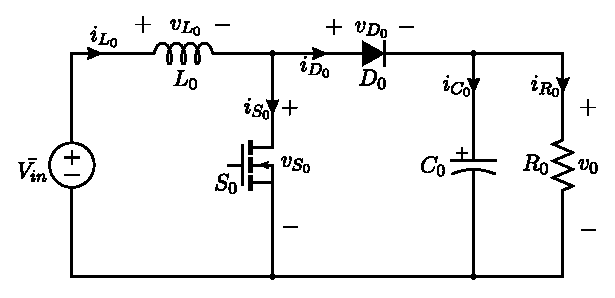
\includegraphics[width=1\linewidth]{Figs/BoostConv}
	\caption{Conversor Boost.}
	\label{fig:boost}
\end{figure}

\subsection{Parâmetros de projeto do conversor Boost}


A \tabref{tab:parametros} apresenta os parâmetros de projeto do conversor Boost.

\textcolor{red}{atualize os valores da tabela, arquivo \emph{Buck\_parametros.tex} }

% Tabela com parâmetros do conversor
% Tabela com parâmetros do conversor
\begin{table}[!ht]
\centering
\caption{Parâmetros de projeto do conversor Boost referente ao registro acadêmico de número $951404$}
\label{tab:parametros}
\begin{tabular}{@{}ccc@{}}
\toprule
\textbf{Símbolo} & \textbf{Descrição} & \textbf{Valor}\\ \midrule
$f_s$ & Frequência de comutação & \SI{15}{\kilo\hertz}\\
$V_i$ & Tensão média de entrada  & \SI{75}{\V}\\
$V_0$ & Tensão média de saída  & \SI{200}{\V} \\
$P_0$ & Potência processada  & \SI{1000}{\W} \\
$R_0$ & Resistência de carga & \SI{40}{\ohm} \\
$\Delta{i_{L_0}}$  & Ondulação de corrente & \SI{40}{\%}\\
$\Delta{v_{C_0}}$  & Ondulação de tensão & \SI{2.5}{\%}\\
$L_0$ & Indutância & \SI{1562.5}{\micro\henry}\\
$C_0$ & Capacitância & \SI{41.6667}{\micro\farad}\\
\bottomrule
\end{tabular}
\end{table}





\section{Verificação do ponto de operação via simulação}

A análise teórica apresentada anteriormente deve ser verificada por simulação \cite{noauthor_psim_nodate}.

A \tabref{tab:steadystate} apresenta o ponto de operação do conversor Boost.
\textcolor{red}{atualize os valores da tabela, arquivo \emph{Buck\_steadystate.tex} }

% Tabela com o ponto de operação do conversor
% Tabela com o ponto de operação do conversor
\begin{table}[!ht]
\centering
\caption{Ponto de operação do conversor Boost referente ao registro acadêmico de número $1721534$}
\label{tab:steadystate}
\begin{tabular}{@{}ccc@{}}
\toprule
\textbf{Símbolo} & \textbf{Descrição} & \textbf{Valor}\\ \midrule
$G$ & Ganho estático & \SI{2.2}{}\\
$D$ & Razão cíclida  & \SI{54.5455}{\%}\\
$I_0$ & Corrente média na carga  & \SI{5.4545}{\A} \\
$I_{L_0}$ & Corrente média no indutor & \SI{12}{\A} \\
$R_a$ & Resistência de medição & \SI{470}{\kilo\ohm} \\
$R_b$ & Resistência de medição & \SI{1}{\kilo\ohm} \\
$H_v$ & Ganho de medição (tensão) & \SI{2.1231}{\milli\V\per\V} \\
$R_s$ & Resistência shunt & \SI{0.1}{\ohm} \\
$H_i$ & Ganho de medição (corrente) & \SI{0.1}{\A\per\A} \\
$V_C$ & Tensão de controle  & \SI{0.54545}{\V} \\
$V_{CM}$ & Tensão máxima de controle  & \SI{1}{\V} \\
$V_{Cm}$ & Tensão mínima de controle  & \SI{0}{\V} \\
\bottomrule
\end{tabular}
\end{table}




A \tabref{tab:steadystatesim} apresenta uma comparação dos valores teóricos com os obtidos por simulação para o ponto de operação do conversor Boost.
\textcolor{red}{atualize os valores da tabela, arquivo \emph{Boost\_steadystatesim.tex} }

% Tabela com o ponto de operação do conversor
% Valores da simulação do ponto de operação do conversor
\begin{table}[!ht]
\centering
\caption{Comparação dos valores teóricos e simulados para o ponto de operação do conversor Boost referente ao registro acadêmico de número $1693832$}
\label{tab:steadystatesim}
\begin{tabular}{@{}cccc@{}}
\toprule
\textbf{Símbolo} & \textbf{Teórico} & \textbf{Simulado} & \textbf{Descrição}\\ \midrule
$I_{L_0}$ & \SI{35}{\A} & \SI{35.0039}{\A} & Corrente média\\
$\Delta{i_{L_0}}$  & \SI{5.25}{\A} & \SI{5.2251}{\A}& Ondulação de corrente\\
$V_{C_0}$ & \SI{150}{\V} & \SI{149.9949}{\V} & Tensão média\\
$\Delta{v_{C_0}}$  & \SI{0.225}{\V} & \SI{0.22706}{\V}& Ondulação de tensão \\
\bottomrule
\end{tabular}
\end{table}



A \figref{fig:boost-steadystate} apresenta a resposta da simulação do ponto de operação do conversor..  \textcolor{red}{compare se os valores simulados com os parâmetros de projeto...}

\begin{figure}[!ht]
	\centering
	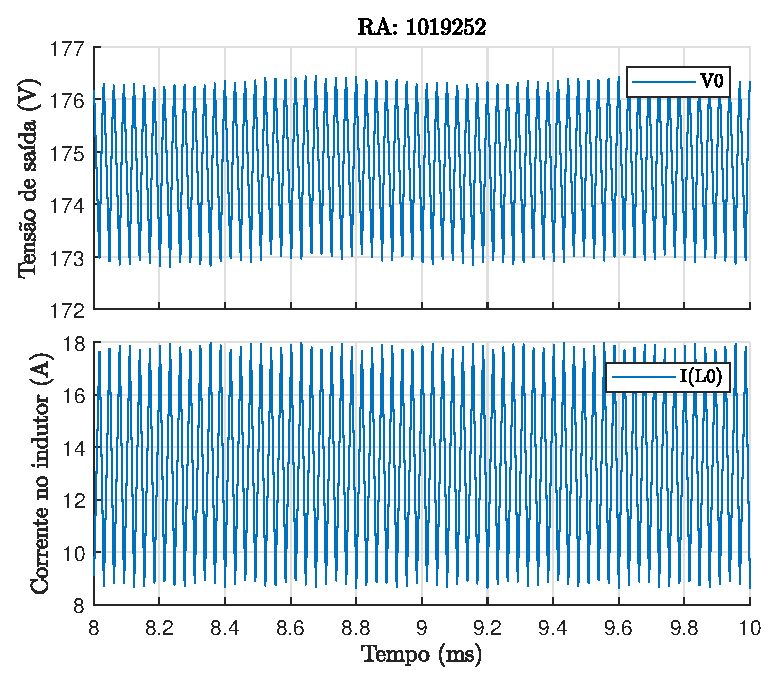
\includegraphics[width=0.9\linewidth]{Figs/Boost}
	\caption{Verificação do ponto de operação do conversor Boost.}
	\label{fig:boost-steadystate}
\end{figure}

\section{Verificação do modelo dinâmico via simulação}


\begin{figure}[!ht]
	\centering
	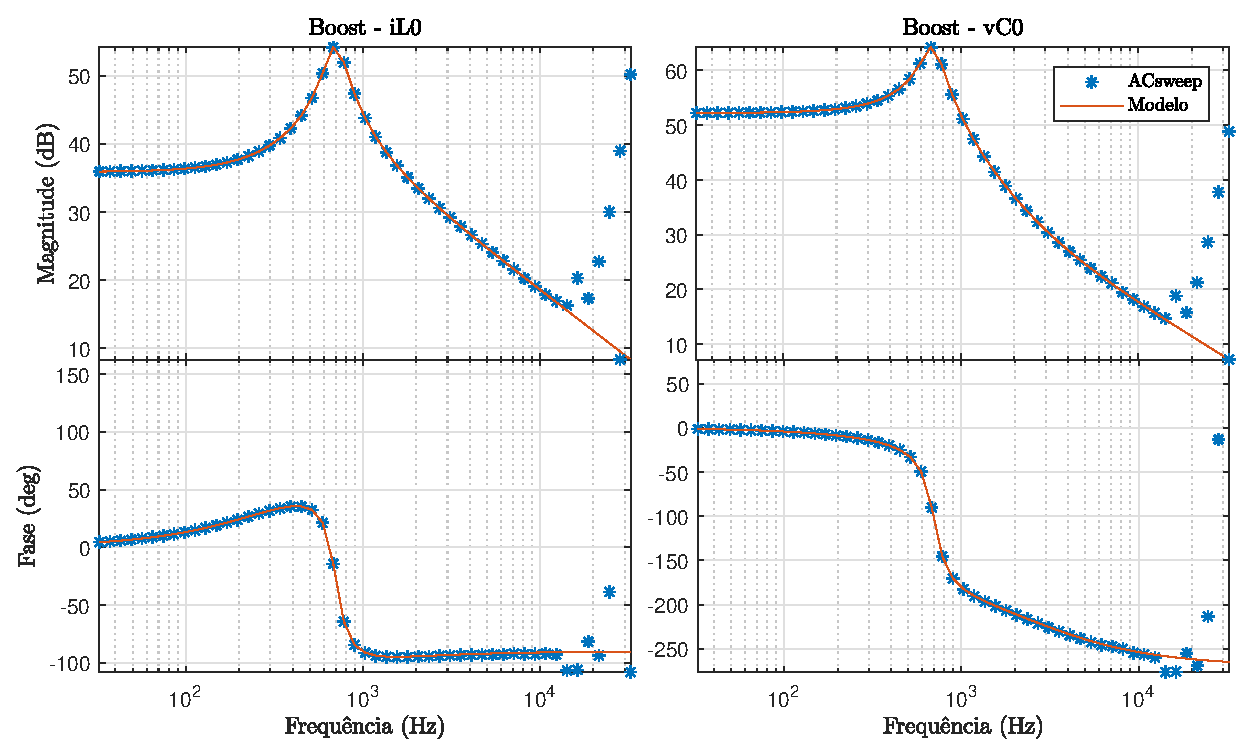
\includegraphics[width=1\linewidth]{Figs/BoostACSweep}
	\caption{Comparação do diagrama de Bode das funções de transferência em função da razão cíclica obtida via simulação no PSIM.}
	\label{fig:ValidacaoModelo}
\end{figure}


\section{Projeto do controlador de tensão}
Detalhes do projeto do controlador de tensão



% Tabela com a resposta ao degrau de referência
% Tabela com resposta ao degrau de referência
\begin{table}[!ht]
\centering
\caption{Resposta ao degrau de referência de tensão $v_{C0}$ do conversor Boost, registro acadêmico de número $1019252$}
\label{tab:resposta1malha}
\begin{tabular}{@{}cc@{}}
\toprule
\textbf{Descrição} & \textbf{Valor}\\ \midrule
Ganho proporcional & \SI{0}{}\\
Ganho integral & \SI{56.1925}{}\\
Margem de ganho & \SI{3.5579}{\deci\bel}\\
Margem de fase & \SI{89.7828}{\degree}\\
Frequência de cruzamento & \SI{75.3985}{\radian\per\s}\\
Tempo de subida & \SI{36.2807}{\milli\s}\\
Tempo de acomodação & \SI{42.484}{\milli\s}\\
Tensão máxima de acomodação & \SI{306.2843}{\V}\\
Tensão mínima de acomodação & \SI{283.8101}{\V}\\
Sobresinal & \SI{0.51875}{\V}\\
Tensão de pico & \SI{306.2843}{\V}\\
Tempo da tensão de pico & \SI{90.8901}{\milli\s}\\
\bottomrule
\end{tabular}
\end{table}



\subsection{Implementação analógica do controlador PI}

% Tabela com a resposta ao degrau de referência
% Tabela com resposta ao degrau de referência
\begin{table}[!ht]
\centering
\caption{Resposta ao degrau de referência de tensão $v_{C0}$ do conversor Buck, registro acadêmico de número $1234567$, implementado com Amplificador Operacional.}
\label{tab:resposta1malhaAmpOp}
\begin{tabular}{@{}cc@{}}
\toprule
\textbf{Descrição} & \textbf{Valor}\\ \midrule
Ganho proporcional & \SI{1.2195e-05}{}\\
Ganho integral & \SI{369.5492}{}\\
Resistor do controlador PI $R_{1_{PI}}$ & \SI{820}{\kilo\ohm}\\
Resistor do controlador PI $R_{2_{PI}}$ & \SI{10}{\ohm}\\
Resistor do controlador PI $C_{1_{PI}}$ & \SI{3.3}{\nano\F}\\
Tempo de subida & \SI{7.406}{\milli\s}\\
Tempo de acomodação & \SI{7.7032}{\milli\s}\\
Tensão máxima de acomodação & \SI{225.8359}{\V}\\
Tensão mínima de acomodação & \SI{215.16}{\V}\\
Sobresinal & \SI{0}{\V}\\
Tensão de pico & \SI{225.8359}{\V}\\
Tempo para a tensão de pico & \SI{18.2535}{\milli\s}\\
\bottomrule
\end{tabular}
\end{table}





\subsection{Implementação digital do controlador PI}

O Código--fonte \ref{lst:valoresPI} atribui os valores das constantes do controlador PI de tensão implementado.
\begin{lstlisting}[caption={Parâmetros do controlador PI digital de tensão.},label={lst:valoresPI}]
// Constantes do controlador
double  a0z = 1.00000000e+00;
double  a1z = -1.00000000e+00;
double  b0z = 5.30305662e-05;
double  b1z = -4.65043351e-05;
\end{lstlisting}
O Código--fonte \ref{lst:implementacaoPI} apresenta a rotina que implementa o controlador PI...
\begin{lstlisting}[caption={Implementação do controlador PI digital de tensão.},label={lst:implementacaoPI}]
e0=in[0]; // Erro atual
// Calcula saída atual 
u0= (e0*b0z+e1*b1z-u1*a1z)/a0z; 
u1=u0; // Atualiza saída anterior
e1=e0; // Atualiza erro anterior    
out[0] = u0; // Saída do controlador
\end{lstlisting}


\subsection{Comparação entre as respostas ao degrau de referência}


\begin{figure}[!ht]
	\centering
	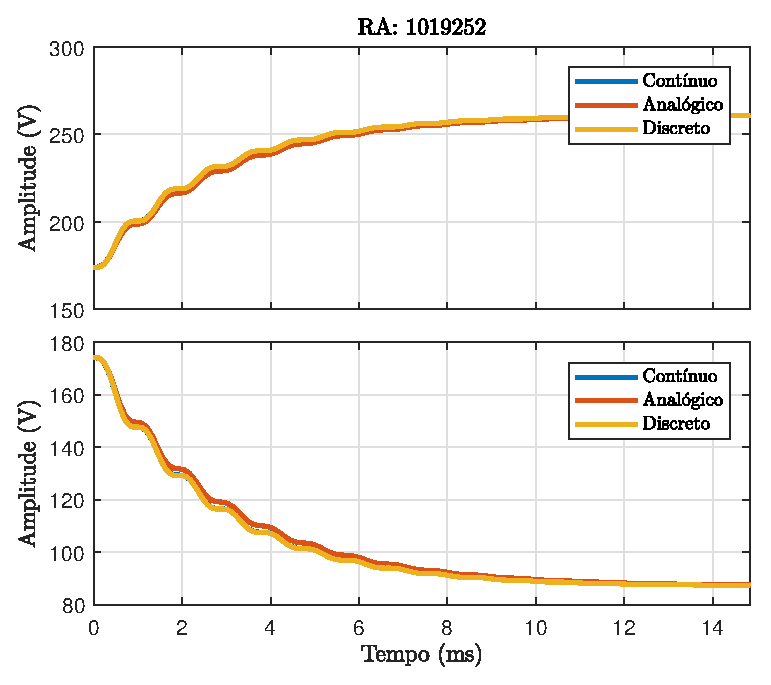
\includegraphics[width=0.9\linewidth]{Figs/BoostStepResponse1malhaTodos}
	\caption{Resposta ao degrau de referência de tensão.}
	\label{fig:stepresponse1malha}
\end{figure}


\section{Implementação com duas malhas}


% Tabela com a resposta ao degrau de referência
% Tabela com resposta ao degrau de referência
\begin{table}[!ht]
\centering
\caption{Resposta ao degrau de referência de tensão $v_{C0}$ do conversor Boost, registro acadêmico de número $1019252$, com controle de duas malhas.}
\label{tab:resposta2malhas}
\begin{tabular}{@{}cc@{}}
\toprule
\textbf{Descrição} & \textbf{Valor}\\ \midrule
Ganho proporcional (controle de corrente) & \SI{0.35678}{}\\
Ganho integral (controle de corrente) & \SI{10461.7785}{}\\
Ganho proporcional (controle de tensão) & \SI{0}{}\\
Ganho integral (controle de tensão) & \SI{368.9346}{}\\
Tempo de subida & \SI{243.1367}{\milli\s}\\
Tempo de acomodação & \SI{247.3912}{\milli\s}\\
Tensão máxima de acomodação & \SI{304.6957}{\V}\\
Tensão mínima de acomodação & \SI{290.1166}{\V}\\
Sobresinal & \SI{0}{\V}\\
Tensão de pico & \SI{304.6957}{\V}\\
Tempo para a tensão de pico & \SI{870.8114}{\milli\s}\\
\bottomrule
\end{tabular}
\end{table}





A \figref{fig:BoostStepResponse2malhas} apresenta o resultado da simulação da resposta ao degrau de referência de tensão....

\begin{figure}[!ht]
	\centering
	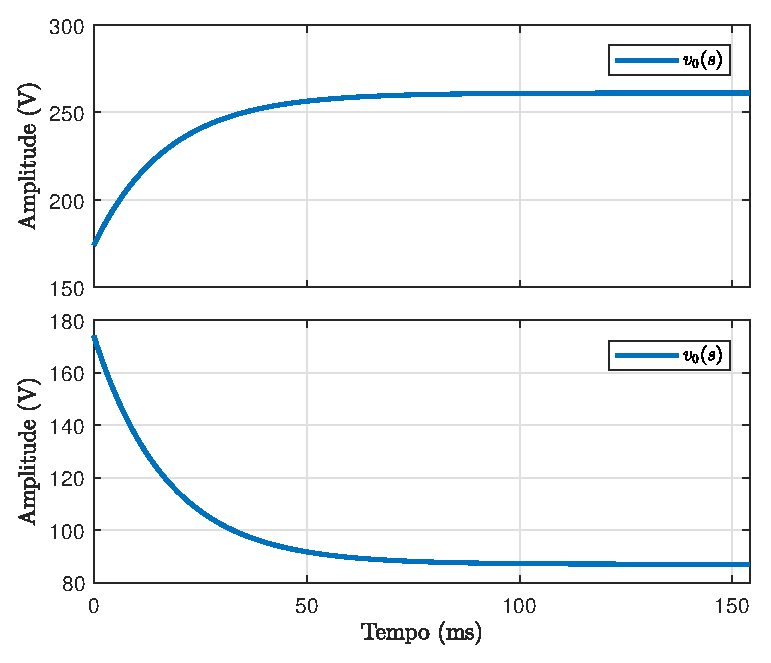
\includegraphics[width=0.9\linewidth]{Figs/BoostStepResponse2malhas}
	\caption{Comparação da resposta ao degrau de referência de tensão para a implementação com uma malha e com duas malhas.}
	\label{fig:BoostStepResponse2malhas}
\end{figure}


A \figref{fig:Buck2malhas} apresenta o resultado da simulação da resposta ao degrau de referência de tensão....

\begin{figure}[!ht]
	\centering
	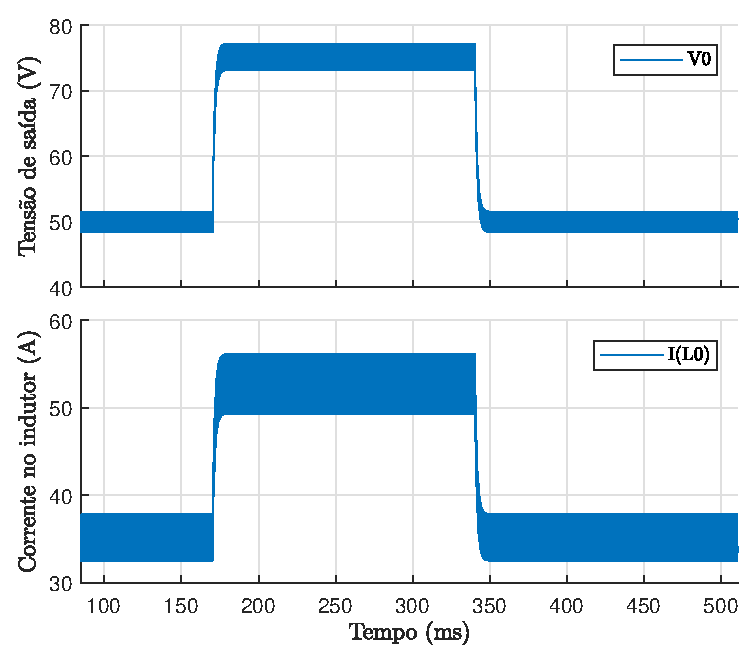
\includegraphics[width=0.9\linewidth]{Figs/Buck2malhas}
	\caption{Resposta ao degrau de referência de tensão com duas malhas de controle.}
	\label{fig:Buck2malhas}
\end{figure}

\section{Conclusões} 


As conclusões devem ser as mais claras possíveis, informando aos leitores sobre a importância do trabalho dentro do contexto em que se situa. As vantagens e desvantagens em relação aos já existentes na literatura devem ser comentadas, assim como os resultados obtidos e as possíveis aplicações práticas do trabalho.


\bibliographystyle{IEEEtran}

\bibliography{Refs/APS} % Inclui arquivos de referência

\balance


